\section{Context-Free Grammar Definition}
A CF grammar is described by $T$, $NT$, $S$, $PR$:
\begin{description}
	\item[$T$:] terminals/tokens of the language;
	\item[$NT$:] non-terminals (sets of strings generated by the grammar;
	\item[$S$:] start symbol ($S \in NT$);
	\item[$PR$:] production roles (indicate how $T$ and $NT$ are combined to generate valid strings).
\end{description}

Derivation is a sequence of grammar rule applications and substitutions (production rules) that transform a starting non-terminal into a sequence of terminals (tokens).
Example:
\begin{lstlisting}
	assign_stmt ::= ID EQ exprs S;
	expr ::= expr operator term;
	term ::= ID;
	term ::= INT;
	...
\end{lstlisting}

\section{How Bottom-Up Parsing Works: Shift/Reduce Technique}
A stack, initially empty, is used to keep track of symbols already recognized.
Terminal symbols are pushed in the stack (shift), until the top of the stack contains a handle (right hand side of a production): the handle is then substituted by the corresponding non-terminal (reduce).
Note that the reduce operation may only be applied to the top of the stack.

Parsing is successful only when at the end of the input stream the stack contains only the start symbol.
Example:
\begin{itemize}
	\item[] input string: ``$a_1, a_2, a_3$''
	\item[] recursive left grammar:
	\begin{lstlisting}
		list ::= list CM EL
		list ::= EL
	\end{lstlisting}
	\item[] scanner: ``$a_1, a_2, a_3$'' $\Rightarrow$ \code{EL CM EL CM EL}
	\item[] parse tree:
	\begin{figure}[H]
		\centerline{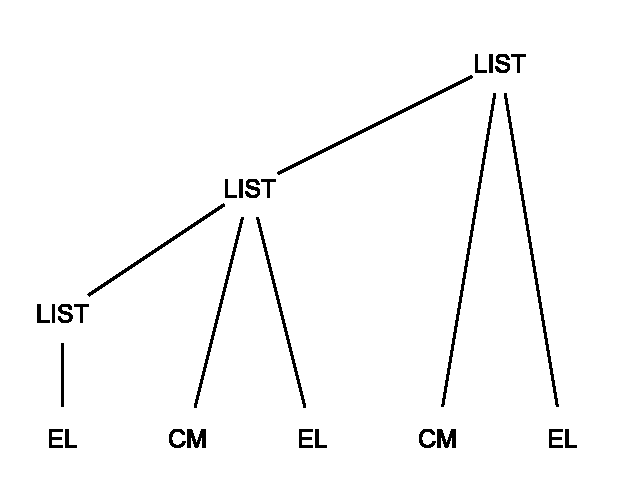
\includegraphics[width=0.5\textwidth]{img/17.pdf}}
	\end{figure}
	\item[] actions:
	\begin{table}[h]
		\centering
		\begin{tabular}{l|l}
			Action & Stack \\ \hline
			 & $\varepsilon$ \\ \hline
			shift & \code{EL} \\ \hline
			reduce & \code{LIST} \\ \hline
			shift & \code{LIST CM} \\ \hline
			shift & \code{LIST CM EL} \\ \hline
			reduce & \code{LIST} \\ \hline
			shift & \code{LIST CM} \\ \hline
			shift & \code{LIST CM EL} \\ \hline
			reduce & \code{LIST} \\ \hline
		\end{tabular}
	\end{table}
\end{itemize}

\section{Introduction to CUP}

\subsection{Source File Format}

\subsection{Setup Section}

\subsection{Terminals/Non-Terminals Section}

\subsection{Rules Section}

\section{Integrating JFlex and CUP}

\subsection{Scanner Modifications}

\subsection{The CUP Parser}

\subsection{Main File (Main.java)}

\subsection{Compiling Steps}